% CS639 final report. Build: cd report && make  (writes ../report.pdf)
\documentclass[11pt]{article}
\usepackage[final]{acl}
\usepackage{times}
\usepackage{latexsym}
\usepackage[T1]{fontenc}
\usepackage[utf8]{inputenc}
\usepackage{microtype}
\usepackage{inconsolata}
\usepackage{graphicx}
\usepackage{booktabs}

\title{LLM Text Detection with Frozen Embeddings and Hypersphere Training Objectives}

\author{Pranshu Dewagan \and Ernie Dippold \and Akshat Jain \and Aviaditya Tamotia \\
  University of Wisconsin--Madison}

\begin{document}
\maketitle
\begin{abstract}
We build a small detector that scores passages as machine-written or human-written without fine-tuning a large language model.
We freeze a sentence embedding model (MiniLM) and train only a linear map into a space where we compare two training objectives: a one-class separation loss and a soft-boundary loss related to Deep SVDD.
We evaluate on the MAGE dataset with ROC AUC, PR AUC, false positive rate at 95\% true positive rate, and accuracy and F1 at a threshold tuned on validation scores.
Soft-boundary training gives modestly better ranking metrics than one-class on our validation split, but both methods still flag many human passages when we insist on catching almost all LLM passages.
\end{abstract}

\section{Introduction}
LLM-generated text shows up in homework, news, and chat, so tools that spot machine-written prose matter for integrity and trust.
Classic supervised classifiers often train on a fixed set of generator models; when a new model appears at test time, accuracy can drop because the model memorized quirks of the old generators rather than a stable ``machine'' signal \citep{zeng2025human,ippolito2019automatic}.

Recent work reframes detection as out-of-distribution (OOD) learning: treat machine text as in-distribution and human text as lying outside a tight region in embedding space \citep{zeng2025human}.
We follow that idea in a lightweight setup.
We encode text with a frozen sentence encoder, add a trainable linear head, and train with hypersphere-style losses so machine embeddings sit closer to a center than human embeddings.
We compare a simple one-class objective to a soft-boundary objective with an adaptive radius.

Our goal is not to beat every published baseline.
We want a clean ablation of the loss function under the same encoder, data slice, and evaluation code, plus plots that explain how scores behave.

\paragraph{Contributions.}
(1) A reproducible PyTorch script that trains both objectives and saves metrics and figures.
(2) Numbers on a stratified MAGE validation slice showing soft-boundary slightly improves ROC and PR curves.
(3) A short discussion of score scale, overlap between classes, and the cost of high recall.

\section{Related Work}
\paragraph{Machine-generated text detection.}
\citet{gehrmann2019gltr} showed that surface statistics and model logits can separate human and machine text in some settings, which motivates richer features than hand counts alone.
\citet{ippolito2019automatic} study automatic detection of machine text and stress that detectors can overfit to specific generators.
The MAGE benchmark \citep{wang2023mage} mixes domains and sources so we can test behavior on heterogeneous text.

\paragraph{OOD detection and SVDD-style models.}
\citet{zeng2025human} treat human-written text as OOD relative to LLM text and train several detectors, including Deep SVDD style objectives and energy-based scores, with strong reported results on large benchmarks.
Deep SVDD \citep{ruff2018deep} learns a representation where normal points stay near a center and anomalies fall away; our soft-boundary hinge and radius update borrow that spirit while we keep the sentence trunk frozen to save compute.

\paragraph{Relation to our codebase.}
We implement the hypersphere head ourselves in \texttt{experiments/objective\_ablation}.
The bundled \texttt{ood-llm-detect-main} folder mirrors the public Zeng et al.\ repository and includes energy and HRN training scripts; we cite it as design reference rather than as the exact code path we ran for the tables below.

\section{Method}
\subsection{Encoder}
For each passage $x$ we compute a vector $e(x)$ with \texttt{sentence-transformers/all-MiniLM-L6-v2} and freeze all encoder weights.

\subsection{Projection and center}
A linear map gives $z(x) = W e(x) + b \in \mathbb{R}^{128}$.
We fix a center $c$ on the unit sphere by averaging projected machine (label 0) training points and normalizing, matching the style used in SVDD demos where the ball describes ``normal'' machine text.

\subsection{Losses}
Let $d^2(x) = \| z(x) - c \|^2$.
Both objectives use a separation term that pushes average $d^2$ lower on machine rows than on human rows within each mini-batch.

The \textbf{one-class} run stops there.

The \textbf{soft-boundary} run adds a hinge on machine rows relative to a radius $R$ in distance units, with hyperparameter $\nu = 0.1$.
After a warm-up of one epoch, we set $R$ to the $(1-\nu)$ quantile of $\sqrt{d^2}$ over all machine training rows, then refresh it at the end of each later epoch.

\subsection{Scores and evaluation}
At test time we want \textbf{higher score} to mean ``more like machine text'' for ROC code.
One-class uses $-d^2$.
Soft-boundary uses $-(d^2 - R^2)$ with the final $R$ from training.

We train for four epochs with AdamW, batch size 48, learning rate $3 \times 10^{-4}$.
We keep the checkpoint with the best validation ROC AUC (not necessarily the last epoch), then report all other metrics on that checkpoint.

\section{Experimental Setup}
\subsection{Dataset}
We load \texttt{yaful/MAGE} from Hugging Face \citep{wang2023mage}.
Label 0 means machine-generated text; label 1 means human-written text.
We randomly subsample 3000 training rows (seed 42), then split by class so 10\% of each class forms validation and the rest trains.
That way validation always contains both labels.

\subsection{Hyperparameters}
Table~\ref{tab:hparams} lists the settings for the run reported in this PDF.
They match the \texttt{--fast} preset in our script.

\begin{table}[t]
\centering
\small
\begin{tabular}{ll}
\toprule
Setting & Value \\
\midrule
Sentence encoder & \texttt{all-MiniLM-L6-v2} (frozen) \\
Projection dimension & 128 \\
Optimizer & AdamW, lr $3{\times}10^{-4}$ \\
Batch size & 48 \\
Epochs & 4 \\
$\nu$ (soft-boundary) & 0.1 \\
Radius warm-up epochs & 1 \\
Train rows used & 3000 (random subset of MAGE train) \\
Validation fraction & 0.1 per class (stratified) \\
\bottomrule
\end{tabular}
\caption{Hyperparameters for the reported experiment.}
\label{tab:hparams}
\end{table}

\subsection{Preprocessing}
We pass raw \texttt{text} strings to the encoder library without extra cleaning beyond its internal tokenization.

\section{Results}
Table~\ref{tab:metrics} summarizes validation metrics at the best ROC epoch (epoch 1 for one-class, epoch 3 for soft-boundary).
Figure~\ref{fig:curves} shows ROC and precision-recall overlays.
Figure~\ref{fig:hists} shows score histograms by class.
Figure~\ref{fig:pca} shows a 2D PCA of the projected vectors $z$ on validation (PCA is unsupervised, so overlap here does not contradict a working threshold in score space).
Figure~\ref{fig:concept} is a toy diagram only; it is not real data.

\begin{table}[t]
\centering
\small
\begin{tabular}{lcccccc}
\toprule
Objective & ROC AUC & PR AUC & FPR@95\%TPR & Acc@F1 & Prec@F1 & Rec@F1 \\
\midrule
One-class & 0.637 & 0.776 & 0.798 & 0.733 & 0.740 & 0.957 \\
Soft boundary ($\nu{=}0.1$) & 0.681 & 0.802 & 0.820 & 0.730 & 0.730 & 0.976 \\
\bottomrule
\end{tabular}
\caption{Validation metrics on the stratified MAGE slice. FPR@95\%TPR is the false positive rate on humans when the threshold is set to reach 95\% true positive rate on LLM text. Acc, Prec, Rec are taken at the F1-optimal threshold on a score quantile grid.}
\label{tab:metrics}
\end{table}

\begin{figure*}[t]
\centering
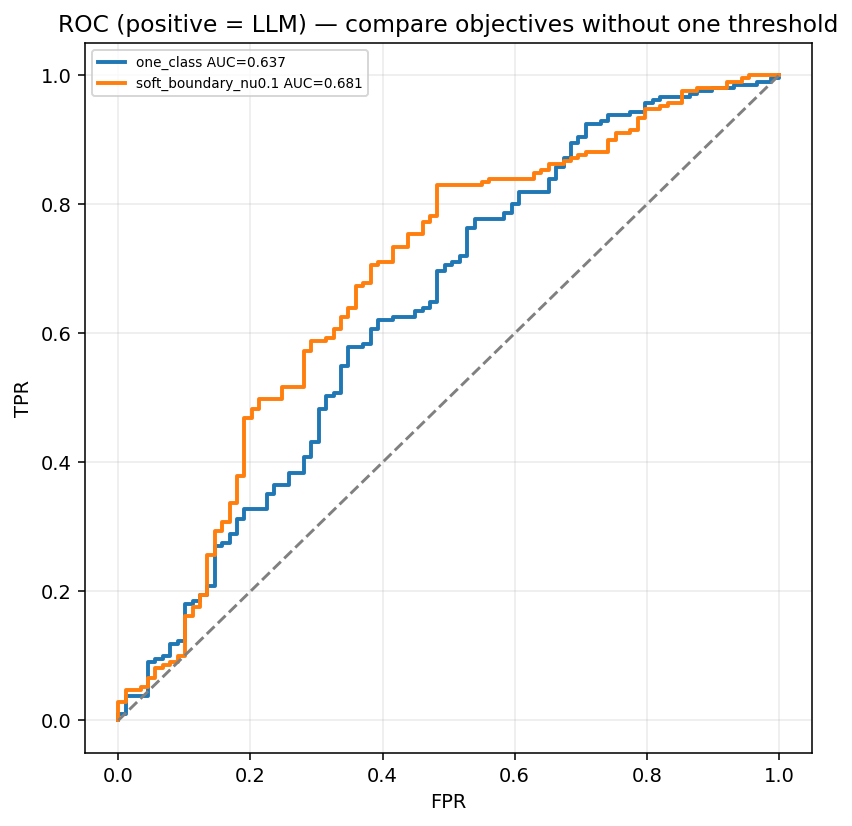
\includegraphics[width=0.46\textwidth]{figures_exp_c/roc_overlay.png}\hfill
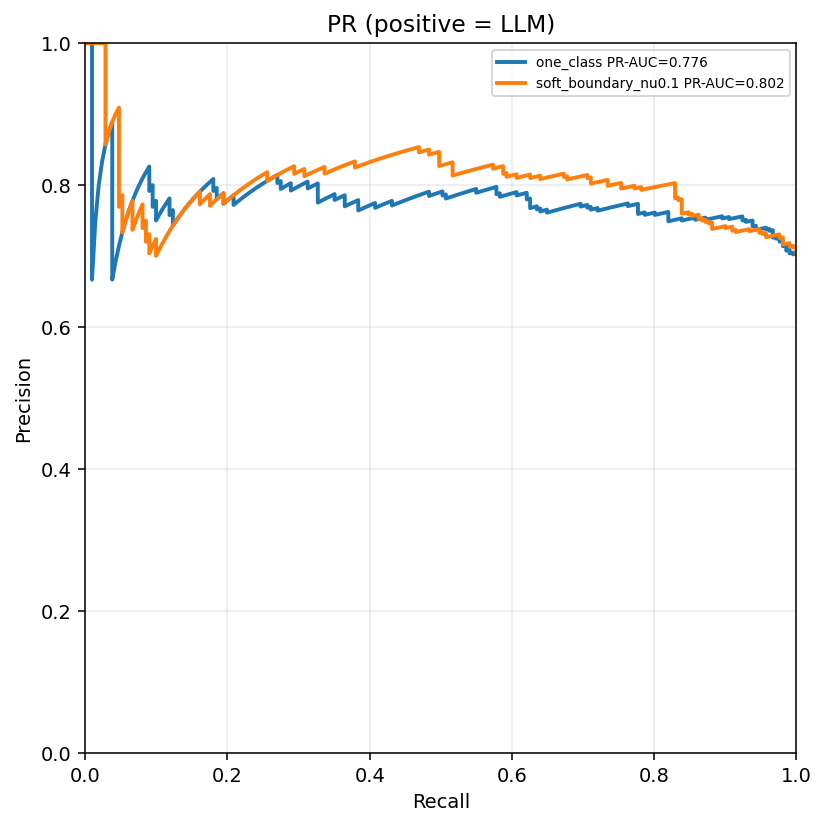
\includegraphics[width=0.46\textwidth]{figures_exp_c/pr_overlay.png}
\caption{Left: ROC curves (LLM positive). Right: precision-recall curves. Soft-boundary (orange) sits above one-class (blue) for most of the range.}
\label{fig:curves}
\end{figure*}

\begin{figure*}[t]
\centering
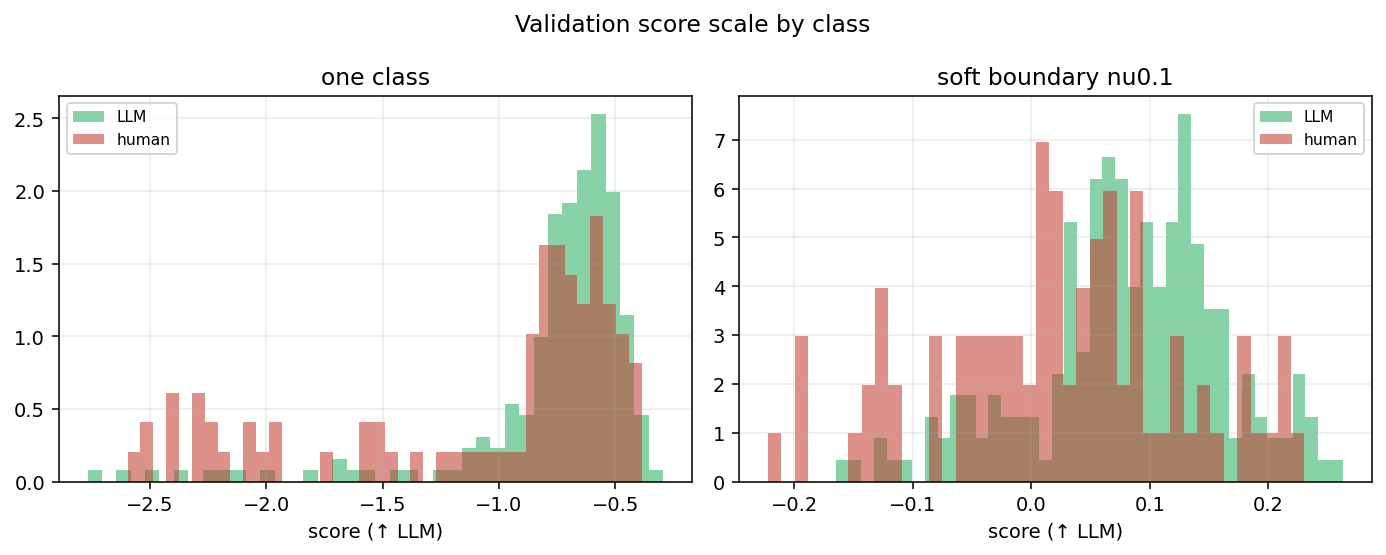
\includegraphics[width=0.46\textwidth]{figures_exp_c/val_scores.png}\hfill
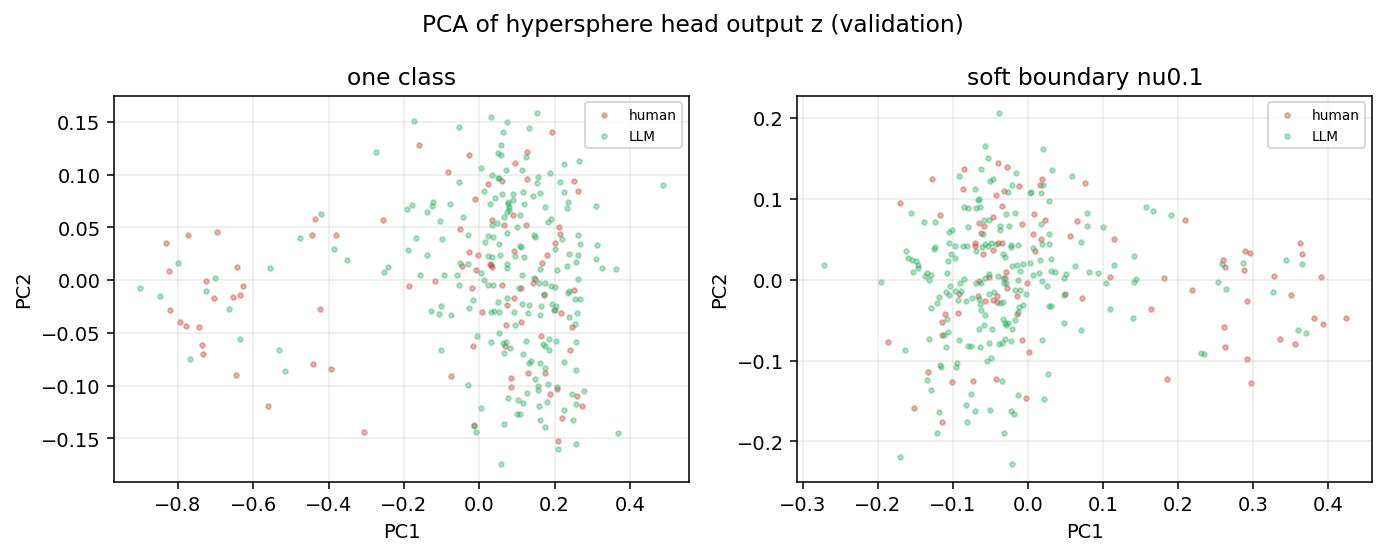
\includegraphics[width=0.46\textwidth]{figures_exp_c/pca_z_val.png}
\caption{Left: validation score densities by true class. Right: PCA of head outputs $z$. Green is LLM, red is human.}
\label{fig:hists}
\end{figure*}

\begin{figure}[t]
\centering
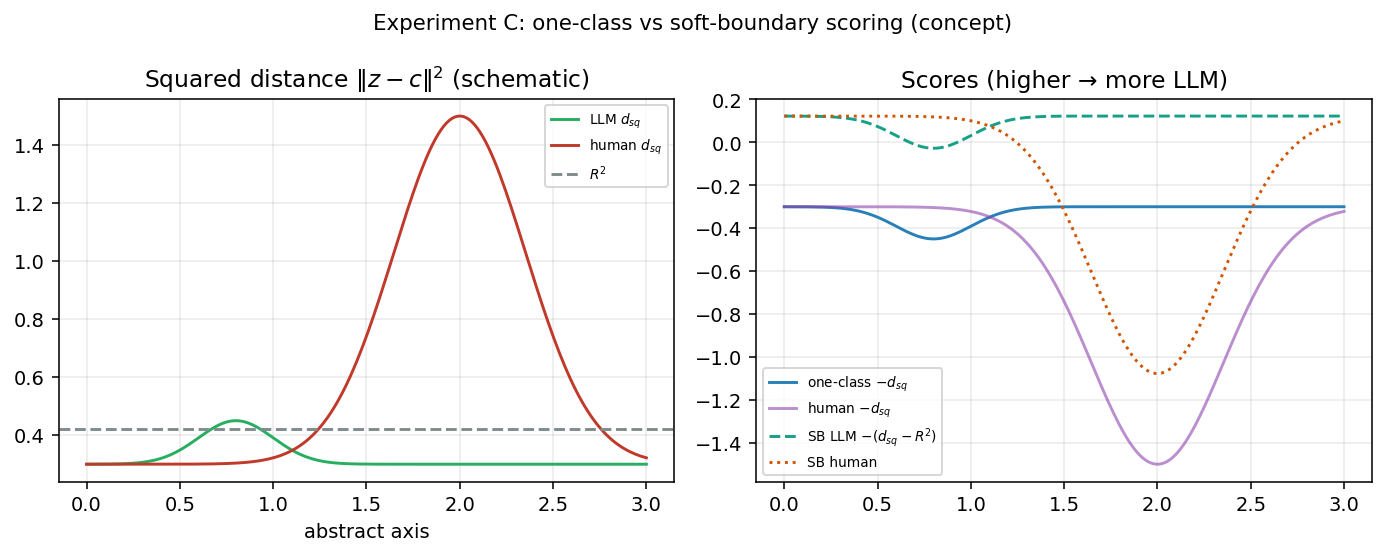
\includegraphics[width=\columnwidth]{figures_exp_c/concept.png}
\caption{Illustrative sketch of squared distance and scoring rules (not from MAGE data).}
\label{fig:concept}
\end{figure}

\subsection{What we observed}
\textbf{Direction of scores.}
For both objectives, mean machine scores sit above mean human scores on validation, which matches the intended ordering.

\textbf{Soft-boundary vs one-class.}
Soft-boundary improves ROC AUC by about 0.04 and PR AUC by about 0.03 on this split.
That is a real but small gap; with only 3000 training rows and four epochs, we should not over-interpret noise.

\textbf{High recall is expensive.}
At 95\% true positive rate on LLM text, the false positive rate on human text stays around 0.80 for both runs.
So a policy that tries to catch almost every machine passage still alarms on most human passages.
That matches the heavy overlap in the histograms.

\textbf{PCA view.}
The first two principal components of $z$ mix classes heavily.
That is expected: PCA does not optimize class separation, and two dimensions miss most of the structure.

\section{Conclusion}
Frozen embeddings plus a small hypersphere head give a simple OOD-style detector we can train on a laptop.
Soft-boundary training slightly improves ranking metrics relative to one-class separation on our validation slice, but neither method fixes the hard tradeoff when we demand very high recall on LLM text.

Limitations: small data slice, short training, single encoder choice, no adversarial or cross-domain stress tests yet.
Future work could add RAID-style attacks, match a teammate energy baseline on the same text file for a fair table, or scale to more MAGE rows and epochs.

\section*{Author contributions}
Pranshu Dewagan: dataset access and subsampling for the group.
Ernie Dippold: figures and polish for the write-up.
Akshat Jain: training code, metrics, scripts, and the run used in this PDF.
Aviaditya Tamotia: testing, review, and repository maintenance.

\section*{Acknowledgments}
Thanks to the course staff and the group for feedback.

\bibliography{references}

\end{document}
